\section{Pyroomacoustics}

In this section we will talk about pyroomacoustics. Pyroomacoustics is a python library developed by EPFL that simulates sound in a room generating the proper echos and decays of sound using omnidirectional sound. 

\begin{figure}[h]
\centering
\begin{minipage}{.5\textwidth}
    \caption{A room with a source at position (1,1)\\ and a circle of microphones centered at (2,2)}
    \centering
    \label{fig:room}
    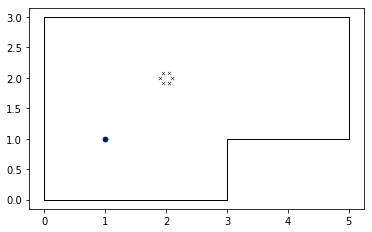
\includegraphics[width=0.8\textwidth]{room.png}
\end{minipage}%
\begin{minipage}{.5\textwidth}
    \caption{The same room but with images of the source to simulate echo}
    \centering
    \label{fig:roomImages}
    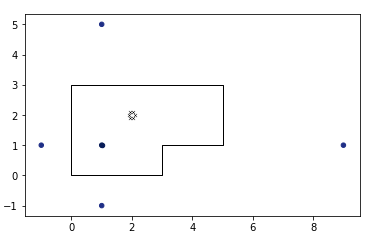
\includegraphics[width=0.8\textwidth]{roomWithImages.png}
\end{minipage}
\end{figure}

What pyroomacoustics do to simulate echo is creating images of the sources out of the room as we can see in figure \ref{fig:roomImages}. These images are created by symmetry with the walls of the room. In order to simulate echo, these images will send the same signal as the source but with a delay and a decay computed with the dirac function and a fractional delay filter \cite{vesaVal}. These signals act as an echo. In the figure \ref{fig:roomImages} we have a first order echo but we could have a second order or even more meaning that it could simulate an echo of an echo etc. We can see the path of these signals sent to the microphones in the figure \ref{fig:roomImagesTrait}

\begin{figure}[h]
\centering
\caption{The room with the path of the signals}
\centering
\label{fig:roomImagesTrait}
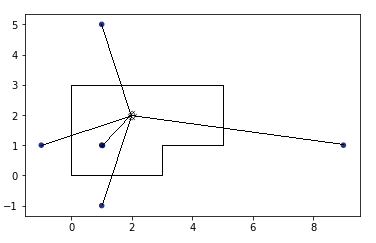
\includegraphics[width=0.5\textwidth]{roomWithImagesAndTrait.png}
\end{figure}

What we wanted to do with pyroomacoustics was to use it and modify the code in order to adapt it to be able to use different impulse responses than the omnidirectional one. So we would be able to use our LEGO and KEMAR responses and see if scattering could help in the direction of arrival for a room with echo. So the microphone class was modified to keep in memory the different impulse responses. And we also modified how the room impulse response was computed in order to take in account the given impulse responses. Another thing we had to think about was which angles to choose when using the impulse responses. Because, as we can see in figure \ref{fig:roomImagesTrait}, the signals come from different directions and the angles from where it comes from probably are not integer values and, even if they are, they might not correspond to an available angle in the impulse responses. Indeed, our impulse response is a discrete response and doesn't include all integer angles also. Meaning that one of the problems we were facing was to interpolate our values so what we decided to do was to take the closest available angle to the computed angle from the positions of the microphones.

Sadly the adaptation done was not working as, when comparing the anechoic case of pyroomacoustics with the music algorithm explained earlier, the results were not similar at all but they should have been. We tried different solutions, for example computing the angle for the group of microphones instead of each microphone because that's how the angle was computed when obtaining the impulse responses. But none of the tried solutions worked and there's still a problem. We think that it might come from the fact that we're using different frames of reference or it might come from an unfound bug in the code. Unfortunately we had no time left to work on that. 

The tables \ref{table:py1} and \ref{table:py2} illustrates the bad results that we were talking about. And even in the anechoic case (order 0 or absorption 1) the results are not good as they should be because they should normally look like the music results that we got before. This fact shows that there is something done wrong either in the data or in the algorithm. 


\begin{table}[H]
   \centering
    \begin{tabular}{|c|c|c|c|c|c|}
      \hline
      Order & absorption & N° Freqeuncies & Error Average & Median & Max Error (Min Error) \\
      \hline
      0 & 1 & 129 & 31.3 & 5.5 & 172 (0) \\
      0 & 1 & 257 & 39.1 & 7 & 165 (0) \\
      0 & 1 & 513 & 34.94 & 9.5 & 143 (0) \\
      1 & 0.8 & 513 & 40.72 & 7 & 163 (0) \\
      1 & 0.5 & 513 & 29.52 & 6.5 & 147 (0) \\
      1 & 0.2 & 513 & 31. & 7 & 169 (0) \\
      2 & 0.5 & 513 & 27.28 & 6.5 & 164 (0) \\
      \hline
    \end{tabular}
    \caption{Summary of pyroomacoustics with a shoe box room with dimensions 10x10. Every line is a compilation of 50 runs each done with a noise of 20 decibel.}
    \label{table:py1}
\end{table}


\begin{table}[H]
   \centering
    \begin{tabular}{|c|c|c|c|c|c|}
      \hline
      Order & absorption & N° Freqeuncies & Error Average & Median & Max Error (Min Error) \\
      \hline
      0 & 1 & 513 & 29.34 & 8 & 149 (0) \\
      1 & 0.8 & 513 & 38.46 & 5.5 & 172 (0) \\
      1 & 0.5 & 513 & 48.34 & 10.5 & 177 (0) \\
      1 & 0.2 & 513 & 35.76 & 6.5 & 170 (0) \\
      2 & 0.5 & 513 & 35.34 & 7.5 & 168 (0) \\
      \hline
    \end{tabular}
    \caption{Summary of pyroomacoustics with a shoe box room with dimensions 20x20. Every line is a compilation of 50 runs each done with a noise of 20 decibel.}
    \label{table:py2}
\end{table}
